\chapter{Análisis previo del problema}
Este capítulo servirá de preludio al capítulo de implementación dando un primer
análisis de los diversos aspectos tanto del problema como del funcionamiento y
estructura de TvTropes, de modo que permita proceder con los primeros
\textit{milestones} del desarrollo del \textit{software} y entender la
estrategia que se seguirá a lo largo del desarrollo con respecto a entender y
resolver el problema. Primero se dará un modelo inicial del problema de
construcción de un \textit{scraper} de TvTropes aplicando el patrón de
\textit{Domain Driven Design}. Luego, se analiza la estructura que sigue la web
de TvTropes, identificando los puntos más importantes para saber cómo abordar la
creación de la araña que explore todas las páginas relevantes de TvTropes y la
extracción de la información que queremos en cada una de ellas. El objetivo
general del capítulo es servir de inicio para saber cómo abordar la solución al
problema y así poder llevarlo luego a lo práctico en la implementación del
\textit{software} en el \autoref{c:6}, en el que se modelarán nuevas partes del
problema conforme se van alcanzando los distintos hitos que permitan llegar a la
solución final.

\section{Modelado inicial del problema}
Con el objetivo de cumplir los dos milestones siguientes, relativos al inicio
del desarrollo del \textit{scraper} que extrae información de películas
(\href{https://github.com/jlgallego99/TropesToGo/milestone/3}{M2} y
\href{https://github.com/jlgallego99/TropesToGo/milestone/7}{M3}), se describe
primero la metodología a seguir para modelar el problema que se pretende
resolver en todo este trabajo y luego se definen las partes básicas de ella para
poder comenzar con el desarrollo en el siguiente capítulo. Al estar en un marco
de desarrollo ágil no se tiene un modelo completo desde el principio, sino que
se necesitarán modelar nuevas y diferentes partes del problema conforme se
avance en el desarrollo. Esto se especificará en el \ref{c:6}, donde se
introducirán progresivamente nuevos elementos al modelo del problema y se irán
resolviendo. Por tanto, en este capítulo se pretende dar un modelo inicial con
el que entender cómo se va a abordar este aspecto del desarrollo y cómo poder
empezar con las primeras etapas de construcción del \textit{software}. El
modelado del problema es una forma de tener una abstracción de las distintas
partes del sistema de modo que haya una relación entendible entre el código, el
problema y sus términos concretos. Con esto se tendrá lo necesario para entender
el dominio del problema y pasar de las historias de usuario a un diseño inicial
del código correctamente modularizado.

El diseño dirigido por dominio (\textit{Domain Driven Design} en inglés,
\textit{DDD} para acortar) es una de las metodologías más populares y efectivas
para modelar un problema en el ámbito de la ingeniería del software
\cite{ddd_golang}. Mediante esta metodología se definen una serie de términos y
patrones para modelar un problema como una abstracción de los componentes
necesarios que puedan manejar el dominio del problema; en este caso, la
extracción de información de TvTropes. Este modelado del problema nos permite
definir las estructuras de datos, interfaces y los posibles errores o
excepciones de forma general en el código que describan todas las partes
importantes del dominio del problema y que luego se implementarán en el
\autoref{c:6}. De esta manera, se definirá un lenguaje unificado que todo el
mundo implicado con este trabajo, tanto usuarios como clientes como
desarrolladores, pueda entender y nos permita referirnos a todos los conceptos
del dominio por términos fácilmente identificables y traducibles a código
\cite{ddd_golang}.

\textit{DDD} define una serie de componentes que permiten dividir el dominio del
problema en contextos muy definidos para facilitar que se creen unidades con
responsabilidad única y que se puedan desarrollar de manera independiente. Los
componentes que utilizaremos en este proyecto para modelarlo son: las entidades,
los objetos valor, los agregados, los repositorios y los servicios
\cite{ddd_golang}. 

Este lenguaje único propicia el código limpio en este desarrollo, ya que,
\textit{DDD} es una metodología que sigue varios de sus principios
\cite{clean_code_rules}; el código sigue una estructura sencilla, bien definida
y comprensible a primera vista, que serían las distinciones de dominio que
define. Además, todos los componentes en \textit{Domain Driven Design} están
relacionados entre sí siguiendo su filosofía, lo que propicia que esas
relaciones se entiendan de primeras. Cada componente del dominio es fácilmente
traducible a un módulo con responsabilidad única que define una serie de
funciones descriptivas, simples y que realizan una sola tarea. Luego, existen
otros componentes llamados servicios que relacionan de forma entendible todas
esas funciones simples para formar un núcleo lógico, manteniendo las relaciones
y flujo de ejecución entendibles y a un alto nivel, sin necesitar de saber cómo
están implementados por dentro.

El principal componente de estudio son las entidades y objetos valor, ya que, el
resto de componentes se deducen de estos. Las entidades son ítems o estructuras
mutables y únicamente identificables que mantienen su identidad a lo largo del
ciclo de vida, pero que pueden cambiar de estado \cite{jannik_ddd}. Por otro
lado, los objetos valor son ítems inmutables no identificables, muy cercanos a
tipos de datos que pueden ser más simples o complejos que, no obstante,
describen las características de algo como una instancia; producir uno implica
instanciar uno nuevo y no modificar el ya existente \cite{jannik_ddd}.

Estos dos conceptos se unen mediante los agregados. Un agregado permite combinar
y encapsular estas entidades y objetos valor, definiendo una interfaz común para
ellos. Están principalmente definidos por una entidad raíz, cuyo identificador
permite identificar al agregado. La lógica de negocio debe estar contenida en
los agregados, que trabajarán con las entidades y objetos valor que la componen.
Se puede entender un agregado como un objeto completo que realiza las
funcionalidades que queremos y en el que sus datos no son accesibles desde
fuera, solamente utilizables desde funciones. Es responsabilidad de las
entidades y objetos valor el representar correctamente su información para que
el agregado los pueda utilizar correctamente \cite{ddd_golang}.

En esta metodología entra también el concepto de repositorio, que almacena o
persiste la información de un agregado, puesto que estos son la unidad de mayor
importancia en \textit{DDD} \cite{ddd_golang}. El repositorio añade una capa de
abstracción para el almacenamiento de datos, generalmente usando el patrón
repositorio, el cual fue introducido por \begin{otherlanguage}{english}Edward
Hieatt y Rob Mee\end{otherlanguage} en el libro
\begin{otherlanguage}{english} Patterns of Enterprise Application Architecture
\end{otherlanguage}\cite{fowler2002eea} y cuyo cometido es mediar entre las
capas de datos y de dominio usando una interfaz que permita acceder a los
objetos del dominio. El repositorio acepta peticiones de objetos cliente del
dominio (que generalmente serán los servicios) y encapsula el código que ejecuta
todas las operaciones sobre la colección de datos, ocultando los detalles de
implementación del almacenamiento, consiguiendo así que la lógica de negocio
funcione de manera independiente. Esto garantiza la propiedad de única
responsabilidad y permite que, en caso de necesitar a lo largo del desarrollo
otro método de persistencia de datos, no haga falta refactorizar todo el código,
sino simplemente modificar el repositorio, manteniendo el resto del código
intacto. 

Se tendrán repositorios encargados de persistir los resultados de la extracción
del \textit{scraper}, es decir, las obras con sus \textit{tropos}, el cual dará
finalmente el producto que el \textit{software} ofrece al usuario para
satisfacer sus necesidades. Para implementar esto en Go es necesario entender su
filosofía de programación. Go no es un lenguaje orientado a objetos; utiliza un
patrón más moderno para la reutilización del código que es el de composición y
no existe el concepto de herencia \cite{debnath_introduction_2022}. Programar en
Go implica seguir sus propias reglas y alejarse de la mentalidad clásica de la
programación orientada a objetos. La principal herramienta de composición en Go
son las interfaces y los \textit{structs}, con las cuales se puede implementar
algo cercano al polimorfismo. Se pueden embeber distintos \textit{structs}
dentro de otros, cada uno con su propia responsabilidad, para formar objetos
compuestos, formando una relación de pertenencia entre \textit{structs}, a
diferencia de las relaciones de herencia. Mientras que un \textit{struct}
permite definir un tipo concreto, una interfaz nos permite definir un tipo
abstracto. En Go una interfaz define una serie de métodos genéricos que abstraen
de cualquier tipo de datos concreto y permiten realizar una misma acción de
distintas maneras. Una interfaz solamente es instanciada cuando un
\textit{struct} implementa todos sus métodos, en cuyo caso se dice que el objeto
cumple la interfaz. 

Visto esto, tiene sentido describir los repositorios usando una interfaz, que no
solo nos dará una definición de las operaciones del repositorio, sino que además
permitirá implementar esa interfaz con distintos \textit{structs} para distintos
repositorios que traten con los datos independientemente de la manera en la que
se persistan. Cada \textit{struct} que implemente la interfaz repositorio con
distintas formas de persistencia será considerado un repositorio, por lo que, se
pueden crear tantos \textit{structs} como almacenes de datos se necesiten de
forma sencilla. Los repositorios deben tener en cuenta también el dominio del
problema, y en este caso están relacionados con la historia de usuario
\href{https://github.com/jlgallego99/TropesToGo/issues/30}{[HU05]} en la que el
investigador expresa la necesidad de poder elegir el formato de representación
para el conjunto de datos, y cada formato de representación de datos será un
repositorio.

Finalmente, queda un componente de \textit{DDD} para terminar de formar las
partes básicas del modelo de la aplicación: los servicios. El concepto de
servicio tiene múltiples significados según el contexto, sin embargo, en esta
metodología hace referencia al componente que orquesta el resto de componentes
que se han definido anteriormente, los cuales están débilmente acoplados y
necesitan de una unidad que los haga funcionar para poder formar la aplicación
que cumpla las necesidades del dominio. El servicio es el principal encargado de
tratar con los repositorios.

Adicionalmente, en el ámbito del \textit{Domain Driven Design} se sugiere el uso
del patrón factoría para la creación de agregados, repositorios y servicios
\cite{ddd_golang}. Por tanto, se tendrán funciones que se encargarán de la
creación de todo el objeto de forma transparente al desarrollador que lo esté
utilizando; no necesita saber qué ocurre sino solamente el objeto correctamente
creado.

Finalmente, se definen los siguientes componentes que modelan los principales
módulos que se tendrán en la extracción de datos en TvTropes, definiendo lo
necesario para entender el dominio del problema a un nivel general y poder
comenzar a desarrollar el \textit{scraper} y conocer las distintas partes que
componen el dominio: las páginas de TvTropes, las obras y los \textit{tropos}.
Todos estos componentes son necesarios para extraer la información de cualquier
página de TvTropes, razón por la que el primer \textit{milestone} del desarrollo
se centra en ello, ya que, su objetivo es dar una primera versión funcional de
un \textit{scraper} básico para TvTropes. A continuación se describen los
componentes \textit{DDD} que permiten modelar esto y poder organizar
inicialmente los distintos ficheros y directorios del código: 
\begin{itemize}
  \item \textbf{Objetos valor:}
  \begin{itemize}
    \item
    \textbf{\href{https://github.com/jlgallego99/TropesToGo/blob/master/tropestogo/trope.go}{\textit{Trope}}},
    el recurso reiterativo en el que se pone el foco en este trabajo. Un
    \textit{tropo} es inmutable, ya que, sigue una denominación concreta que
    provee TvTropes y, aunque cada uno es único, están definidos por su nombre y
    descripción. Si se le cambiase la descripción o nombre a un \textit{tropo}
    resultaría en uno distinto, que casaría con la idea de que en este ámbito de
    estudios surgen constantemente nuevos \textit{tropos}, a veces relacionados
    con anteriores, pero que son distintos.\\
    En el ámbito de este trabajo definimos que una obra está definida por sus
    \textit{tropos}, describen un aspecto del dominio, lo que hace que estos
    sean objetos valor. Al ser un objeto valor, se tratará únicamente
    instanciándolo, se representará como un \textit{struct} en Go y sus campos
    serán privados, accesibles desde funciones. 
  \end{itemize}
  \item \textbf{Entidades:}
  \begin{itemize}
    \item
    \textbf{\href{https://github.com/jlgallego99/TropesToGo/blob/master/tropestogo/page.go}{\textit{Page}}},
    concretamente las páginas de las obras, que contienen toda una estructura
    HTML y se identifican unívocamente por su URL. Sus características pueden
    cambiar, ya que, la comunidad puede modificar o añadir nuevos datos a ella
    en cualquier momento y se debe tener en cuenta para satisfacer la historia
    \href{https://github.com/jlgallego99/TropesToGo/issues/9}{[HU04]}, en la que
    se especifica la necesidad de tener la información lo más actualizada
    posible. Estas páginas hacen referencia a todas las páginas de obras de
    cualquier medio audiovisual, puesto que, es lo que pide el usuario
    (\href{https://github.com/jlgallego99/TropesToGo/issues/6}{[HU01]}).
    Adicionalmente, el \textit{scraper} necesitará toda la información del HTML
    para poder analizarla, por lo que debe estar codificada como un árbol DOM
    que permita recorrerlo. Una página de TvTropes debe almacenar solamente el
    HTML que le interesa al usuario atendiendo a las
    \href{https://github.com/jlgallego99/TropesToGo/issues/6}{[HU01]} y
    \href{https://github.com/jlgallego99/TropesToGo/issues/7}{[HU02]}. Esto se
    verá más en profundidad en la siguiente sección, donde se analizará la
    estructura de una página de TvTropes.\\
    Al ser una entidad, se tratará desde los agregados como una referencia
    (utilizando punteros), ya que, cada una de las páginas mantiene su identidad
    según su URL y va cambiando.
    \item
    \textbf{\href{https://github.com/jlgallego99/TropesToGo/blob/master/tropestogo/work.go}{\textit{Work}}},
    es la denominación en TvTropes para una obra audiovisual, independientemente
    del medio al que pertenezca. En el dominio del problema, una obra evoluciona
    en el tiempo conforme sus \textit{tropos} cambian y, además, está
    identificada por su título. Si tuviese otro título sería una obra distinta,
    por tanto, se llega a la conclusión de que esto es una entidad.\\
    Al igual que las páginas, las obras también se tratarán desde los agregados
    como referencias mediante punteros, manteniendo su identidad.
  \end{itemize}
  \item \textbf{Agregados:}
  \begin{itemize}
    \item
    \textbf{\href{https://github.com/jlgallego99/TropesToGo/blob/master/tropestogo/index/index.go}{\textit{Index}}}:
    Relacionado con la funcionalidad del \textit{crawler}, se encarga de indexar
    las entidades página de TvTropes, para que luego el siguiente agregado, el
    \textit{scraper}, extraiga su información. La entidad raíz de este agregado
    será la página. Los índices se deben persistir en un repositorio para
    cumplir la historia de usuario
    \href{https://github.com/jlgallego99/TropesToGo/issues/9}{[HU04]}, que
    especifica que la información debe estar actualizada, por lo que, el
    propósito de este agregado es obtener las páginas que no se tienen y
    actualizar las que ya están registradas, sin caer en peticiones redundantes.
    \item
    \textbf{\href{https://github.com/jlgallego99/TropesToGo/blob/master/tropestogo/media/media.go}{\textit{Media}}}:
    Relacionado con la funcionalidad del \textit{scraper}, extrae el conjunto de
    todos los \textit{tropos} de todas las obra que pertenecen a un medio
    audiovisual (llamado \textit{media} en inglés y en TvTropes) concreto. La
    entidad raíz en este caso será la obra, de la que cuelgan sus
    \textit{tropos}. Pretende cumplir las dos primeras historias de usuario
    \href{https://github.com/jlgallego99/TropesToGo/issues/6}{[HU01]} y
    \href{https://github.com/jlgallego99/TropesToGo/issues/7}{[HU02]}, que piden
    que se obtenga toda la información de \textit{tropos} o un subconjunto de
    ellos. Una obra con sus \textit{tropos} debe tener además información
    adicional de metadatos que permita distinguirla de otras con mismo nombre
    para cumplir la
    \href{https://github.com/jlgallego99/TropesToGo/issues/8}{[HU03]} y saber lo
    actualizada que está para cumplir
    \href{https://github.com/jlgallego99/TropesToGo/issues/9}{[HU04]}. El
    agregado se asegurará, por tanto, de que se tienen todos los \textit{tropos}
    existentes en una obra y permitiendo poder elegir tanto la obra u obras como
    el medio, con posibilidad de extraerlo todo o una parte. Este agregado se
    encargará de extraer los datos de TvTropes y dar una API para dar acceso a
    la principal unidad que pretende conseguir este trabajo: la obra con sus
    \textit{tropos}.
  \end{itemize}
  \item \textbf{Repositorios:}
  \begin{itemize}
    \item Un repositorio que almacene el
    \href{https://github.com/jlgallego99/TropesToGo/blob/master/tropestogo/index/repository.go}{indexado}
    de las páginas relevantes de TvTropes para su posterior extracción,
    identificar si ha cambiado su contenido y no estar constantemente haciendo
    peticiones a la web
    (\href{https://github.com/jlgallego99/TropesToGo/issues/9}{[HU04]}).
    \item Adicionalmente, uno o más repositorios que persistan el
    \href{https://github.com/jlgallego99/TropesToGo/blob/master/tropestogo/media/repository.go}{conjunto
    de datos} en varios formatos
    (\href{https://github.com/jlgallego99/TropesToGo/issues/30}{[HU05]}).
  \end{itemize}
  \item \textbf{Servicios:}
  \begin{itemize}
    \item El
    \textbf{\href{https://github.com/jlgallego99/TropesToGo/blob/master/tropestogo/service/crawler/crawler.go}{\textit{Crawler}}}
    será el servicio encargado de controlar el flujo del agregado
    \textit{Index}. Identificará e indexará las páginas de TvTropes que se
    necesitan y las almacenará en un repositorio para persistir el resultado del
    \textit{crawling} y no sobrecargar la red con numerosas peticiones a la
    misma página, ya que, ya se tendrá extraída en su totalidad de forma bruta.
    \item Por otro lado, el
    \textbf{\href{https://github.com/jlgallego99/TropesToGo/blob/master/tropestogo/service/scraper/scraper.go}{\textit{Scraper}}}
    será el servicio que interaccione con el repositorio que contiene las
    páginas indexadas para analizarlas y extraer la información que se busca,
    que finalmente se almacenarán en uno o varios repositorios pertenecientes a
    los distintos almacenes de datos que se definan. 
  \end{itemize}
\end{itemize}

\section{Análisis de TvTropes}
Un wiki complejo como TvTropes, en el que tanto la estructura concreta de una
página como entre ellas cambia bastante, contiene información que es de difícil
acceso y está desperdigada por distintos lugares. A veces, no existe siquiera.
Es por esto que a continuación, tras haber visto cómo se pretende modelar el
problema y organizar el código para poder empezar con las primeras fases del
desarrollo, se estudian los problemas y particularidades que tiene TvTropes y
que queremos resolver con el \textit{scraper} para poder extraer toda la
información que sea posible de la manera más sencilla y eficiente. Esto nos
permitirá resolver los dos primeros \textit{milestones}, donde se analizará y
entenderá la estructura de una página y se extraerá exactamente la información
que se quiere, además de dar información adicional que sirva para entender
TvTropes en general y poder aplicarlo en siguientes hitos. Para ello, se estudia
la organización de las páginas de TvTropes tanto entre sí como dentro de ellas,
y se observan los puntos más importantes que el bot debe saber identificar para
poder desarrollar una estrategia en el siguiente capítulo conociendo todos los
puntos relevantes de la web.

Primero, se hará una breve introducción sobre cómo funciona TvTropes en general.
Luego, se analizará la organización entre páginas para el desarrollo del
\textit{crawler} o araña. Finalmente, se analizará la estructura del código HTML
dentro de una misma página, para el desarrollo del \textit{scraper}.

\subsection{Vista general de TvTropes}
Antes de pasar a entender en profundidad cómo están relacionadas las partes de
TvTropes, es necesario primero ver cómo funciona la web en general y qué
contenidos ofrece.

En este trabajo el interés principal está en identificar y extraer los
\textit{tropos}, que son la principal fuente de información de TvTropes,
conocidos en inglés y en la propia web como \textit{tropes}. Pero además,
TvTropes trabaja con otra información que también se puede considerar como
principal y a la que se accede desde la barra de navegación superior de la
página. Para el ámbito de este trabajo, el más importante es el \textit{Media},
que son los trabajos que existen en un medio audiovisual concreto y que
contienen unos \textit{tropos} asociados. Existe otra sección, la de índices,
que es muy relevante para el estudio de la web en este capítulo y qué se verá en
la siguiente sub sección. Además de esto están otros que no consideramos para el
\textit{scraper}, como el foro o los vídeos.

Una página que describe un \textit{tropo} suele presentar, generalmente, una
descripción de cómo funciona, ejemplos de obras que los tienen organizados por
distintos índices y una lista de sub \textit{tropos} relacionados con él. Que en
una obra aparezca un \textit{tropo} no significa que necesariamente aparezcan
los relacionados con él. Como ejemplo está
\begin{otherlanguage}{english}\textit{TheChosenOne}\end{otherlanguage}, que
presenta como uno de sus sub \textit{tropos}
\begin{otherlanguage}{english}\textit{The Antichrist}\end{otherlanguage}, sin
embargo, no todas las obras en las que aparezca un personaje que es el elegido
tiene por qué ser el anticristo.

Por otro lado, las páginas de obras, aunque visualmente parecidas, presentan
otra información. Al igual que con los \textit{tropos}, lo primero que tienen es
el título y un resumen con información general de la obra, \textit{tropos}
referenciados, enlaces a vídeos, y muchas otras que varía muchísimo entre
páginas. Además de esto, está la parte más importante: una lista de los
\textit{tropos} principales que la comunidad ha identificado, con su
correspondiente descripción, y generalmente presentados de múltiples formas que
dificultan su extracción y que se analizará más en profundidad a lo largo de
este capítulo. Otro aspecto muy destacable en una página de una obra es que
contiene múltiples sub páginas que presentan nuevos \textit{tropos} de ese
trabajo desde otros puntos de vista, personajes, curiosidades, citas, etc.

Además de las secciones vistas, en la barra de navegación superior existe una
barra de búsqueda en la que buscar por nombre el \textit{tropo} u obra
audiovisual en la que esté interesado el usuario y una sección para gestionar
una cuenta de usuario. Las cuentas de usuario no son necesarias para consultar
TvTropes; se emplean para contribuir a la comunidad tanto en el foro como en la
creación de nuevos \textit{tropos}, por lo que se salen fuera del ámbito de este
trabajo y el \textit{scraper} no las tiene que tener en cuenta. Esto además
facilita ciertos aspectos legales, ya que, al tener toda la información
disponible públicamente y sin tener que pasar por la creación de una cuenta que
tenga una serie de condiciones asociadas, permite que el bot pueda recoger esa
información sin mayores consideraciones.

\subsection{El indexado en TvTropes}
Para construir una buena araña que sea capaz de explorar todas las páginas de
TvTropes es necesario entender cómo están relacionadas entre sí las páginas.
Para esto es necesario conocer cómo funciona el indexado en TvTropes, es decir,
de qué manera están organizadas todas las secciones de la web y cómo un usuario
puede encontrar lo que quiere. Al saber cómo un usuario puede encontrar lo que
quiere, también sabemos cómo debe comportarse el \textit{crawler} para indexar
las páginas que necesitamos.

La araña necesita un buen punto de partida a partir del cual, indexando todos
los hipervínculos que encuentre, pueda ir explorando recursivamente y encontrar
todas las páginas que necesita luego el \textit{scraper}. Todos los
\textit{tropos} están listados en un índice llamado \textit{Main}. En él se
puede ver que todos los \textit{tropos} siguen en su URL la misma forma que
consiste en \texttt{https://tvtropes.org/pmwiki/pmwiki.php/Main/} más el nombre
del tropo en estilo \textit{CamelCase}. Sin embargo, existen páginas de este
estilo que no son tropos, sino que son nuevos índices que sí que desembocan en
\textit{tropos} finalmente. Además, el saber la URL no sirve para encontrarlos,
antes se necesita saber cuáles existen y sus nombres.

Existe dos índices de \textit{tropos} que los ordenan alfabéticamente. Uno de
esos índices\footnote{\url{https://tvtropes.org/pmwiki/index_namespaces.php}} da
una barra de búsqueda en la que poder escribir el nombre del tropo que se busca
y una lista que, sin embargo, no contiene ni mucho menos todos los
\textit{tropos}. Al buscar, por ejemplo, aquellos que empiecen por la letra Z
vemos que únicamente se listan tres, mientras que con una breve búsqueda en
cualquier obra se puede ver que hay muchísimos otros con la letra Z que no están
listados. Esto evidencia que en este índice faltan muchos \textit{tropos} y no
puede usarse como un buen punto de partida para ellos. Por suerte, existe otro
índice que sí que los contiene
todos,\footnote{\url{https://tvtropes.org/pmwiki/pagelist_having_pagetype_in_namespace.php?n=Main&t=trope}}
ya que, es un script interno de TvTropes que hace una búsqueda en toda la web
con páginas de un tipo llamado \textit{trope}. Por tanto, se debería tener en
cuenta este último porque nos asegura que están listados todos los existentes en
la página y además es el que se recomienda en los
foros\footnote{\url{https://tvtropes.org/pmwiki/posts.php?discussion=14420393930A40584600&page=1}}.

Por último, se puede observar que la URL de este último índice contiene
parámetros que, si se modifican, nos permiten obtener un índice completo de, por
ejemplo, todas las
películas\footnote{\url{https://tvtropes.org/pmwiki/pagelist_having_pagetype_in_namespace.php?n=Film&t=work}}
o todos los
videojuegos\footnote{\url{https://tvtropes.org/pmwiki/pagelist_having_pagetype_in_namespace.php?n=Videogame&t=work}}.

Dirigir la búsqueda de las obras desde los \textit{tropos} no es eficaz ni
correcto, debido a que, la sección de ejemplos de obras dentro de la página de
un \textit{tropo} presenta solo los casos más relevantes y rara vez todas las
ocurrencias existentes. Por tanto, tiene más sentido encontrarlos desde la
propia página de la obra, que será más profunda y completa. La existencia de
unos índices completos donde encontrar todas las páginas de cualquier tipo
permite que la exploración dentro de una página concreta sea únicamente para
extraer información y no hipervínculos para que la araña indexe, así que entra
en el dominio del \textit{scraper}. Además de esto, generalmente las páginas de
\textit{tropos} y obras están constantemente referenciándose mutuamente, y eso
llevaría a bucles difícilmente controlables.

Estos índices también permiten evitar errores observables en el repositorio de
\textit{Tropescraper}, en el que algunos usuarios reportan que existen páginas
que el \textit{scraper} considera como tropos, pero que no lo son. Un ejemplo de
esto es \begin{otherlanguage}{english}\textit{Films of the
2020s}\end{otherlanguage}\footnote{\url{https://tvtropes.org/pmwiki/pmwiki.php/Main/FilmsOfThe2020s}},
en el cual se listan películas a partir del año 2020 y no es un \textit{tropo}
pese a colgar del índice \textit{Main}.

Hasta ahora se ha hablado principalmente del índice de \textit{tropos}, y se ha
visto que se puede utilizar para obtener también un índice con todas las
películas o todos los videojuegos. Sin embargo, estos son solo dos de los tipos
de obras más reconocibles, lo que en TvTropes se conoce como
\textit{media}\footnote{\url{https://tvtropes.org/pmwiki/pmwiki.php/Main/Media}}.
Este índice es bastante complejo porque TvTropes hace una gran separación entre
los trabajos u obras según el medio en el que se presentan. Por ejemplo, en la
categoría de animación distingue entre animación occidental, animación asiática
o anime japonés, o en la categoría de películas distingue entre películas de
acción real o películas de animación. Tropescraper extraía únicamente todas las
películas del índice \textit{Film}, lo que llevaba a dejarse muchas obras que
también son películas, como puede ser El Viaje de Chihiro, que está en la
sección de anime. En este trabajo se usarán las categorías de \textit{media} tal
y como se definen en TvTropes al ser imposible diferenciar, por ejemplo, una
serie de anime de una película anime al estar las dos bajo la misma sección de
anime. En general, estas categorías son subjetivas, por lo que no hay una
solución concreta, sin embargo, se busca poder extraer la información de todos
los tipos de \textit{media} posibles.

Existen índices que agrupan las obras por otros criterios como el género de la
obra, sin embargo, estos son más generales y dividen de forma más ambigua y
subjetiva las obras. Esto, sumado a que atendiendo a los \textit{user journey}
especificados y a la
\href{https://github.com/jlgallego99/TropesToGo/issues/6}{[HU01]}, nos permite
saber que los usuarios quieren el conjunto de datos por tipo de obra y es, por
tanto, el índice que la araña debe explorar, lo cual se verá más en profundidad
a continuación. Adicionalmente, en el caso de necesitar el género de la obra,
podrán extraerlo de fuentes más fiables como IMDB atendiendo a la
\href{https://github.com/jlgallego99/TropesToGo/issues/8}{[HU03]}.

En resumen, se han podido encontrar índices que sabemos con toda seguridad que
contienen todos los tropos y obras separadas por medio, por lo que esto supone
un muy buen punto de partida para la araña y ya mejoraría a
\textit{Tropescraper}, el cual tenía como punto de partida la entrada de la wiki
de \textit{tropos} y \textit{películas}, que no contiene todas las entradas
existentes y son páginas más difíciles de explorar al tener que entrar en sub
índices según género o tipo de media.

\subsection{Organización de las páginas de TvTropes}

TvTropes es una web muy compleja que, aunque su principal objetivo sea listar y
explicar \textit{tropos}, proporciona adicionalmente una gran cantidad de
información para los fans sobre las obras audiovisuales que contiene. Para
seguir profundizando en lo relativo al estudio de esta web, es necesario
analizar el sitio completo, es decir, estudiar cómo se relacionan sus páginas
más relevantes entre sí de una forma entendible. En su
\textit{sitemap}
\footnote{\url{https://tvtropes.org/pmwiki/pmwiki.php/Sandbox/Sitemap}} se
pueden encontrar todas las páginas PHP que dividen las páginas en secciones y
cómo funcionan sus URL. No todas las páginas de TvTropes nos interesan, en
concreto este trabajo está interesado únicamente en las páginas de obras y
\textit{tropos} según las historias de usuario
\href{https://github.com/jlgallego99/TropesToGo/issues/6}{[HU01]} y
\href{https://github.com/jlgallego99/TropesToGo/issues/7}{[HU02]}.

En la figura \ref{fig:sitemap} se representa un mapa del sitio de TvTropes como
un multi grafo dirigido, donde se pueden ver principalmente las páginas que
necesita la araña, aunque también aparecen otras en gris que, aunque no son
necesarias para cumplir con las necesidades del usuario, se representan con el
objetivo de dar un esquema fiel de la web y sus partes principales. Los enlaces
entre ellas se representan mediante flechas que indican la dirección de
navegación y se añaden algunas características adicionales como el patrón de la
URL o la información que se puede encontrar. Esta representación permite poder
entender cómo programar luego la araña para que entienda todo el sitio y sepa en
qué páginas tiene que buscar enlaces que le permitan avanzar a otras páginas
para encontrar todo lo que busca sin perder nada. Es necesario tener en cuenta
que este es un esquema general que no representa todas las páginas; es posible
que, por ejemplo, un índice tenga una página intermedia antes de llegar a un sub
índice, a diferencia de las otras que están en su mismo nivel. En general se
debe tener en cuenta que la navegación entre páginas puede tener excepciones a
las que se observan en este diagrama y que, en caso de ser necesarias para la
araña, se estudiarán y justificarán en el capítulo de implementación al
detectarlas durante el desarrollo.

\begin{figure}[!h]
  \centering
  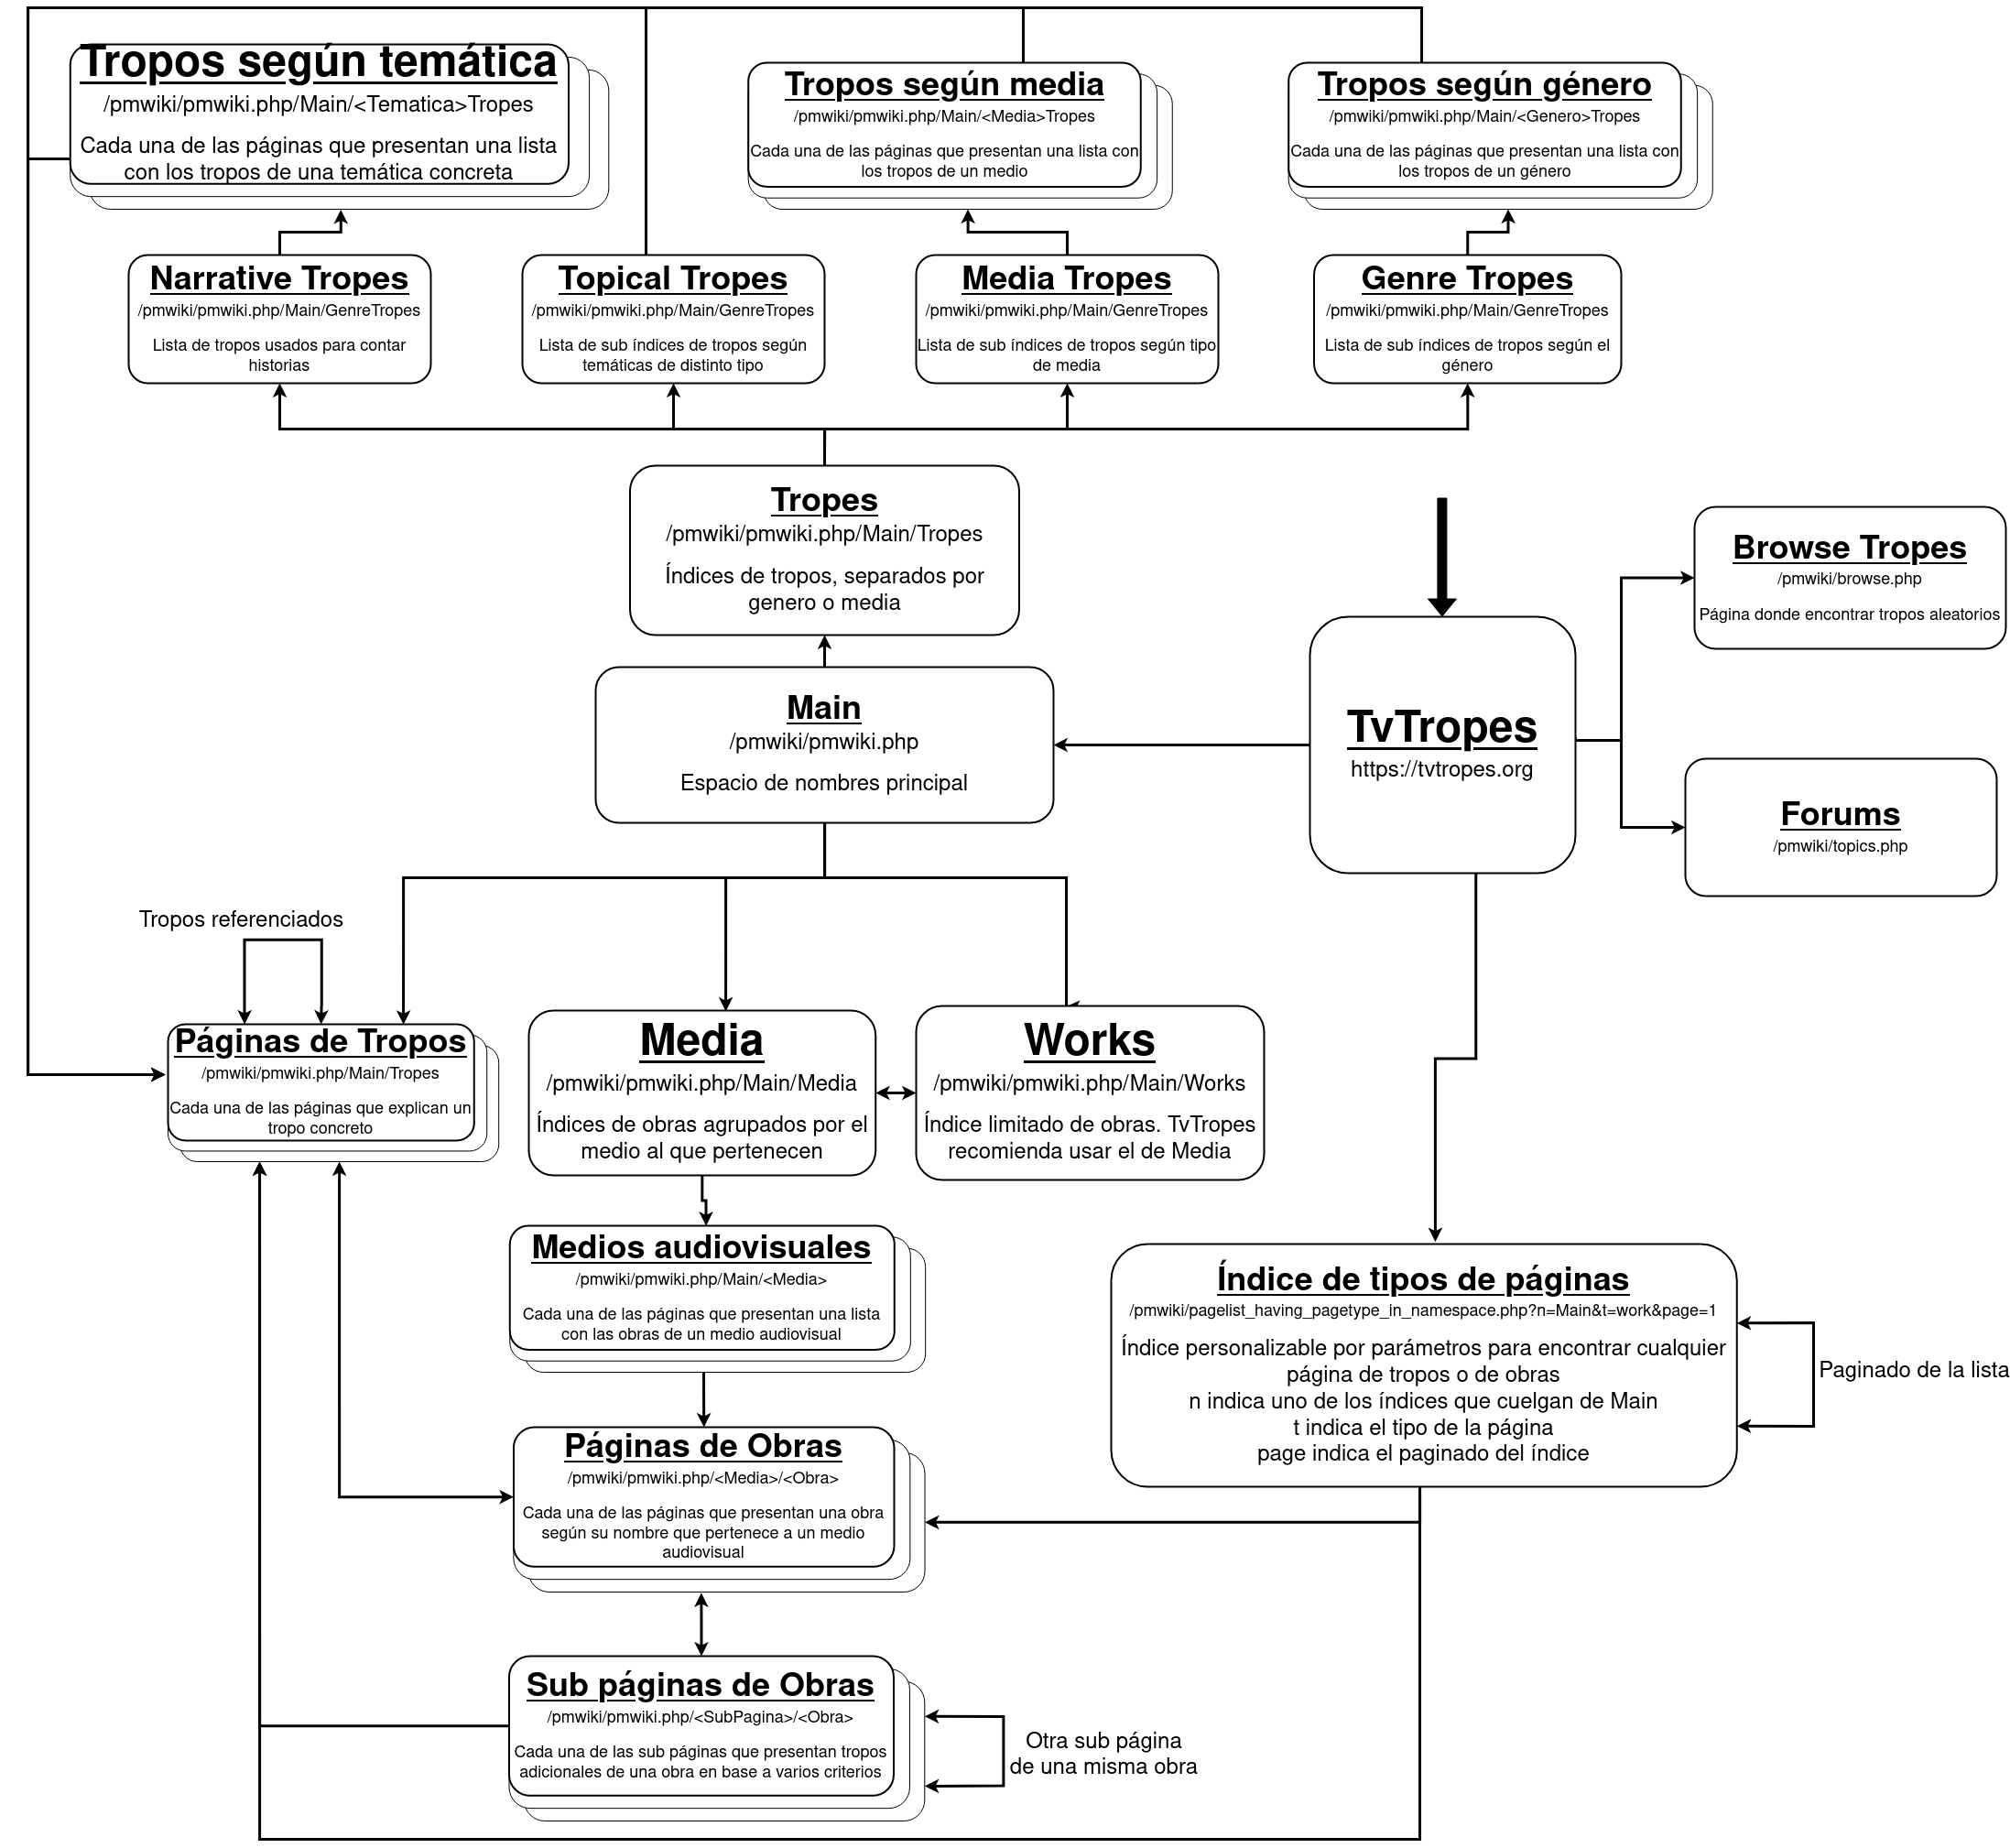
\includegraphics[width=\textwidth]{img/sitemap.png}
  \caption{Mapa del sitio de TvTropes.}
  \label{fig:sitemap}
\end{figure}

Las relaciones más destacables que se pueden observar en el mapa del sitio son
las siguientes:
\begin{itemize}
  \item De \textit{Main} cuelgan la gran mayoría de páginas e índices que debe
  explorar la araña. Existen muchas páginas individuales sin relación entre
  otras y con información que no se han representado al no ser necesaria para
  este trabajo, representando diversos aspectos de la web como la comunidad,
  guías de estilo, información, etc. Estas páginas siguen la misma filosofía que
  las de obras, presentándolas de la misma manera e incluso asociando
  \textit{tropos} a aspectos como el funcionamiento de la propia web, que da a
  ver aún más lo centrales que son estos recursos en esta web.
  \item Existen páginas que, si bien son del mismo tipo, tienen contenidos
  distintos según el contexto, como las páginas de \textit{tropos}, de obras, de
  los distintos índices de \textit{tropos} o de los distintos índices de obras.
  Se han representado como tres rectángulos uno encima de otro para simplificar
  el diagrama, pero todos ellos hacen referencia a que existen muchas páginas de
  esa clase, y no es posible representarlas todas con sus nombres específicos.
  Por ejemplo, la página de una obra dependerá de qué obra represente, y lo
  mismo con los \textit{tropos}. Los índices de \textit{tropos} según temática,
  medio, género o tópico incluyen páginas como \textit{tropos} del género de
  acción o de aventuras, de miedo, de películas, videojuegos o de cualquier otro
  método de organización.
  \item Como se ha explicado antes, existen índices para explorar todos los
  tropos o las obras por tipo de medio. Los índices que aparecen en el mapa del
  sitio, que dependen de \textit{Main}, no son fiables, debido a que no suelen
  contener todas las obras existentes en la web y muchas veces enlazan a índices
  que no tienen que ver. Por ejemplo, es bastante común ir al índice de
  animación asiática y encontrarse con multitud de películas o series que caen
  en la categoría de animación general o en algo completamente distinto como
  animación occidental. Esto hace que sea más fiable saber el índice al que
  pertenece una obra desde dentro de la misma obra y teniendo en cuenta el
  índice principal visto.
  \item Por tanto, el índice más fiable es el que se representa con el nombre de
  índice de tipos de páginas, que es el que se ha visto en la sección anterior.
  Es el más ideal para encontrar todas las páginas porque nos permite listar
  todos los \textit{tropos} u obras según los distintos índices a los que
  pertenecen sin perder ninguno, y navegar hacia cualquiera de ellos, como
  indica la flecha unidireccional. Para navegar dentro del índice hay que tener
  en cuenta que la lista que presenta está paginada, de ahí la flecha de
  navegación hacia sí mismo, ya que, para que la araña explore todo el índice
  debe explorar en profundidad esa página, utilizando el enlace de pasar a la
  siguiente parte de la lista que hay abajo del todo.
  \item Hay relaciones que no se representan al no ser necesarias, como por
  ejemplo que desde la página principal se puede navegar directamente a
  cualquiera de las páginas relevantes de \textit{tropos} u obras, ya sea
  mediante la barra de búsqueda o mediante enlaces que van cambiando
  dinámicamente, ya que, la página destaca cada día nuevas páginas relevantes de
  rápido acceso.
  \item Los \textit{tropos} se están referenciando entre sí constantemente por
  lo que navegar desde uno hacia otro puede ser un proceso interminable. La
  araña puede encontrar otros \textit{tropos} explorando las distintas sub
  páginas de una obra. Las sub páginas, como pueden ser Trivia o YMMV, están
  también representadas como un conjunto genérico, ya que, pueden tomar muchos
  nombres y temáticas. Es importante saber que están siempre enlazadas a la obra
  sobre la que hablan, y no se puede navegar a la de otra obra distinta. Desde
  ellas solo se puede navegar o a otra sub página (siempre de la misma obra en
  la que nos encontramos), a la página principal de la obra o a la página de un
  \textit{tropo} que tiene referenciado en cualquier sub página. Sin embargo,
  cuando desde una página de un \textit{tropo} se referencia a una obra, es
  siempre a la principal.
\end{itemize}

En resumen, desde el índice principal se puede navegar a cualquiera de las
páginas de obras, que pertenecen a un índice de medio audiovisual. Estos medios
audiovisuales se pueden encontrar en el índice principal en \textit{Main}, y
todas las obras están relacionadas únicamente con uno de ellos. Desde la obra se
puede acceder a dos tipos de páginas: sub páginas de la obra y páginas de
\textit{tropos}. Las sub páginas, a su vez, también están relacionadas con los
\textit{tropos}, por lo que se puede navegar hacia ellos desde ahí. Por último,
dentro de una página de \textit{tropos} también se puede navegar hacia otras que
están referenciadas. En general existen una relación casi bidireccional entre
obras y \textit{tropos} al estar referenciándose continuamente. 

\subsection{Estructura de las páginas de TvTropes}
Por último, se analiza la estructura que tiene cada página de TvTropes, tanto de
un \textit{tropo} como de una obra audiovisual, ya sea película, serie,
videojuego, etc. al ser lo que piden las historias de usuario principales
\href{https://github.com/jlgallego99/TropesToGo/issues/6}{[HU01]} y
\href{https://github.com/jlgallego99/TropesToGo/issues/7}{[HU02]}. Se intentan
definir los tipos de páginas más comunes e importantes, pero no todos los que
puedan existir. Es imposible predecir todas las formas que puede tomar una
página, y además eso haría que el \textit{scraper} no supiese adaptarse y fuese
demasiado rígido \cite{nishalscraping}. En general, en esta última sección se
busca identificar las partes más destacables del código HTML de las páginas para
que el \textit{scraper} sepa dónde tiene que buscar la información que necesita
sin redundancia. Este análisis del código HTML se realiza usando las
herramientas de desarrollador presentes en cualquier navegador web, que permiten
observar todo el código HTML de la página, activar o desactivar el JavaScript
para observar los cambios en ella, y demás funcionalidades útiles que sirven en
el ámbito del \textit{scraping} y para sacar conclusiones de las páginas.

Las páginas de obras audiovisuales, independientemente del tipo, se tratan
esencialmente igual y podrían presentar las mismas diferencias que dos del mismo
tipo, sin embargo, suelen tener secciones adicionales. Por ejemplo, si la página
es de una película, es probable que contenga la lista de actores, cosa que por
ejemplo no pasará en un libro o videojuego generalmente, no obstante, en general
entre los cambios que se pueden observar al buscar dos páginas que hacen
referencia a un mismo tema como puede ser dos obras audiovisuales el propósito
es el mismo: describir la obra y sus \textit{tropos}.

Por ejemplo, la página de la serie Los
Soprano\footnote{\url{https://tvtropes.org/pmwiki/pmwiki.php/Series/TheSopranos}}
presenta varias características interesantes, como por ejemplo que el
\textit{tropo}
\begin{otherlanguage}{english}\textit{GenreDeconstruction}\end{otherlanguage}\footnote{\url{https://tvtropes.org/pmwiki/pmwiki.php/Main/GenreDeconstruction}}
no está presente en la sección de \textit{tropos}, que está organizada en cuatro
carpetas según el rango alfabético, sino que se encuentra referenciado en la
propia descripción de la serie. También se pueden encontrar otros
\textit{tropos} que, si bien no están en la propia lista, se les hace referencia
en la descripción de un \textit{tropo} concreto que sí que está en la lista. Al
entrar en otra página, como la de la película El Viaje de
Chihiro\footnote{\url{https://tvtropes.org/pmwiki/pmwiki.php/Anime/SpiritedAway}},
podemos ver que la información ha cambiado por completo de forma y ahora los
\textit{tropos} no se presentan en carpetas y no están organizados por género o
cualquier otra idea, simplemente están en una lista ordenada alfabéticamente.
Por último, es interesante observar una página más, la de la serie
Hannibal\footnote{\url{https://tvtropes.org/pmwiki/pmwiki.php/Series/Hannibal}},
que aunque inicialmente puede parecer que tiene la misma estructura que la de
Los Soprano con cuatro carpetas por rango alfabético, observamos que esos rangos
son distintos. Esta última serie también evidencia otro problema de estructura
que es necesario resolver, y es que existen otras entradas en TvTropes que
también se llaman Hannibal, haciendo referencia o al personaje o a la novela, y
que tienen distinta manera de presentar sus tropos. Sin embargo, cada una de
estas páginas tienen un tipo definido en la web (personaje, serie, libro,
película, etc.) por lo que son más fácilmente identificables.

Como se ha explicado antes, estos cambios estructurales y de organización están
presentes también entre páginas con distintos propósitos, como por ejemplo, en
la página de un \textit{tropo} y de una obra. La página de una obra concreta
muestra los \textit{tropos} organizados en carpetas o listas con distintas
organizaciones, mientras que una página de un \textit{tropo} concreto como el
visto anteriormente de
\begin{otherlanguage}{english}\textit{GenreDeconstruction}\end{otherlanguage} da
la información inversa, es decir, todas las obras que tienen ese \textit{tropo}.
Sin embargo, en este caso la información está presentada de una forma
completamente distinta, esta vez requiere de una mayor exploración a fondo,
puesto que, se dan una serie de géneros con un hipervínculo a sub páginas que
cuelgan de la principal del \textit{tropo} y que ya sí que listan las obras.

En la figura \ref{fig:tvtropes-work} se representan las partes de una página de
una obra en TvTropes que el \textit{scraper} debe saber identificar, ya que
contienen la información que necesitamos. En color azul se muestran las
secciones donde se encuentra información relevante, en verde se muestran las
partes en las que posiblemente se quiera extraer el enlace y/o deban explorarse
más en profundidad y, por último, en rojo se destacan partes no importantes o
que sirven para separar otras que sí son relevantes. Varias de estas partes se
pueden identificar fácilmente en el HTML, puesto que, usan unas etiquetas,
clases e identificadores que siempre son los mismos al ser parte de cómo
funciona internamente la wiki y no contenido que escriben la comunidad. A
continuación se describen estas partes y cómo el \textit{scraper} puede
tratarlas:

\begin{figure}[!h]
  \centering
  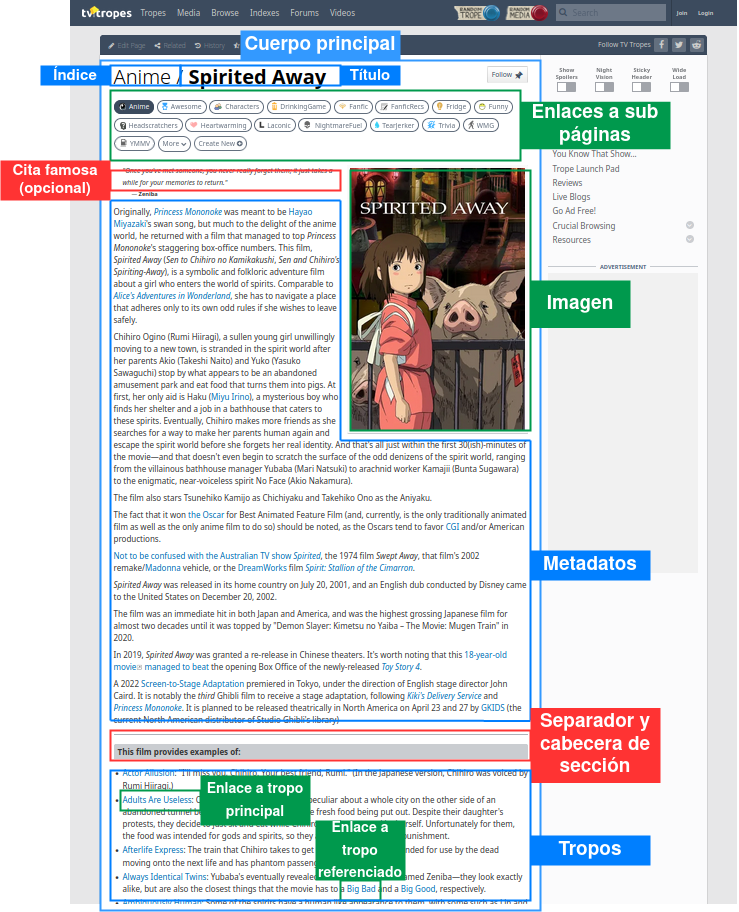
\includegraphics[width=\textwidth]{img/esquema-obra.png}
  \caption{Esquema de las secciones de la página de una obra en TvTropes.}
  \label{fig:tvtropes-work}
\end{figure}

\begin{itemize}
  \item El cuerpo principal es siempre un elemento
  \begin{otherlanguage}{english}\texttt{<article
  id=``main-entry''>}\end{otherlanguage} que nos permite identificar fácilmente
  el cuerpo principal independientemente del tipo de página.
  \item La primera parte del cuerpo principal es siempre una cabecera de sección
  \begin{otherlanguage}{english}\texttt{<h1
  class=``entry-title''>}\end{otherlanguage}. La cabecera contiene en el mismo
  texto el nombre del índice y el título de la obra separados por una barra. El
  nombre del índice siempre está marcado con énfasis, contenido en una etiqueta
  \texttt{<strong>} que lo diferencia del título. Esta diferenciación permite
  conocer a qué índice pertenece cualquier obra.
  \item La sección de enlaces a sub páginas es un poco más compleja; está
  siempre contenida en un elemento de navegación
  \begin{otherlanguage}{english}\texttt{<nav
  class=``body-options''>}\end{otherlanguage} que tiene dentro una lista sin
  ordenar \begin{otherlanguage}{english}\texttt{<ul
  class=``subpage-links''>}\end{otherlanguage}. Dentro de la lista, cada
  etiqueta \texttt{<li>} contiene un hipervínculo a la sub sección de la obra,
  que contendrá otros \textit{tropos} referenciados. En el caso de que una
  página tenga muchos enlaces a sub páginas, no todos se mostrarán directamente,
  y el último botón será un desplegable con el resto. No hace falta usar
  JavaScript para interaccionar con esta parte, ya que, el resto de sub
  secciones que no cabían siguen contenidas ahí. Concretamente, están contenidas
  en el último elemento de lista, que tendrá dentro una etiqueta
  \texttt{<select>} donde cada opción tiene como valor una cadena de texto con
  la ruta URI de la sub página.
  \item A veces, entre las sub páginas y el resumen con metadatos aparece una
  sección con una cita de la obra que se puede ignorar.
  \item Cada obra tiene un resumen, a veces más largo y a veces más corto, que
  cuenta las características principales que tiene. Esta sección es una fuente
  de metadatos difícil de identificar al ser un texto en lenguaje natural, sin
  embargo, también suele contener \textit{tropos} referenciados mediante un
  elemento de hipervínculo. Es posible que parte de los metadatos se encuentren
  separados del resumen, en otro elemento que contenga el texto distinto o
  dentro de una carpeta. Esa carpeta, al igual que con la de \textit{tropos},
  simplemente cambia el texto a visible, por lo que, está en el HTML base y no
  hace falta sacarla de ninguna manera. El resumen está delimitado por un
  elemento \begin{otherlanguage}{english}\texttt{<div
  id=``main-article''>}\end{otherlanguage}, cuyo contenido suele ser muy diverso
  no solo en texto sino en elementos HTML que contiene. Generalmente, los
  distintos párrafos del texto están contenidos en etiquetas \texttt{<p>} o de
  otros tipos. Lo importante aquí es extraer el texto, independientemente de
  dónde esté contenido.
  \item La sección que más interés tiene en cada página de una obra es la de sus
  \textit{tropos}. Antes de esta parte suele aparecer una cabecera que, como se
  vio en \cite{nishalscraping}, tiene un texto que suele cambiar, pero siempre
  suele ser una etiqueta \texttt{<h2>} precedida de una barra horizontal
  \texttt{<hr>} que lo separa del resumen. La sección de los \textit{tropos}
  suele cambiar de forma. A continuación se estudiará más en profundidad cómo
  encontrar los \textit{tropos} en una página de este tipo.
  \item Los marcadores que indican que empieza una sección de \textit{tropos}
  (la línea horizontal y la cabecera) no siempre están presentes. Además, en
  otros casos de páginas, pueden introducir una sección que no contenga
  \textit{tropos}, como pueden ser los actores de una película. En este caso,
  habrá que analizar correctamente las listas e hipervínculos, buscando solo
  aquellos que se sepa que hacen referencia a un \textit{tropo}, que es de la
  página \textit{Main} de TvTropes.
\end{itemize}

En general, los \textit{tropos} pueden aparecer en casi cualquier parte dentro
de la página de una obra y estar organizados de distintas maneras. Algunas los
tienen organizados en una lista o por carpetas en orden alfabético, de géneros o
cualquier otro método de diferenciarlas. También puede haber información de
\textit{tropos} anidada dentro de otros, referenciados en la descripción de la
obra, o incluidos en sub páginas de distinta índole.

En la figura \ref{fig:tropelist} se pueden ver los tres tipos más comunes para
presentar la lista de \textit{tropos} de una obra que se pueden encontrar en
TvTropes. En el primero de la figura \ref{fig:tropelist1} se tiene simplemente
una lista en la cual el primer elemento de cada ítem de la lista es una etiqueta
llamada \texttt{<a class=``twikilink''>} con el nombre del \textit{tropo}, la
clase que ya se ha identificado anteriormente y un enlace a la página de ese
\textit{tropo}. También se puede observar como en la descripción aparecen
enlaces a otros \textit{tropos} que no salen en la lista. El segundo tipo, en la
figura \ref{fig:tropelist2}, es muy parecido al primero solamente que esta vez
están separados en distintas listas, que suelen cambiar el rango alfabético
según la página. Estas carpetas se abren haciendo clic sobre ellas y, mediante
un \textit{script} de JavaScript, aparece la lista de \textit{tropos}, sin
embargo, lo único que hace ese \textit{script} es mostrar la lista modificando
el parámetro CSS de visibilidad. La lista no se inserta dinámicamente, sino que
se pone visible o invisible, por lo que el código HTML base tiene todas las
listas ya definidas independientemente de si están visibles o no. Por último, la
figura \ref{fig:tropelist3} muestra el tipo más complejo y que no es tan común.
Suele aparecer en las obras más famosas, que por lo general tienen un gran
número de \textit{tropos} que hacen que la lista esté contenida en una sub
página y se acceda mediante un enlace en la principal. La dificultad en este
tipo está en que la araña tiene que profundizar en la búsqueda, accediendo a sub
páginas. La ruta de estas será del tipo \texttt{/<NombreDeLaObra>/Tropes<XtoY>}
al final de la URL de TvTropes. En ella, \texttt{<XtoY>} representa un rango
alfabético, siempre precedido por la palabra \textit{Tropes}. Además, estos
enlaces son siempre elementos de primer nivel en la lista, ya que, pueden
aparecer otros que no tienen que ver directamente con los \textit{tropos} y se
pueden ignorar. Una vez entrado en el enlace, la forma de presentar la lista
puede ser de cualquiera de los otros dos tipos vistos.

En el caso concreto de que estén organizados en carpetas, cada una de ellas está
contenida en una etiqueta \texttt{<div>} con un identificador \texttt{folderX}
donde \textit{X} a veces es un número y otras veces puede ser cualquier otra
cosa, generalmente la palabra \textit{label}. En general no siguen una
nomenclatura muy uniforme, pero sí es común que sean etiquetas del mismo tipo y
que empiecen por \textit{folder}. 

Independientemente de cómo se presenten, al final todas las listas que contienen
\textit{tropos} son listas en el lenguaje HTML. Siempre empiezan con una
etiqueta \texttt{<ul>} y cada uno de sus elementos se presentan primero con el
elemento \texttt{<li>} y luego con el enlace que incluye el nombre del
\textit{tropo}. Es bastante usual que, incluso si no están presentados por
carpetas y visualmente parecen una sola lista uniforme, internamente sean varios
elementos \texttt{<ul>} distintos. Las listas siempre están precedidas de una
etiqueta \texttt{<hr>} que pone una línea horizontal y un título \texttt{<h2>}
en el que, como se vio en \cite{nishalscraping}, varía el texto, aunque es
bastante frecuente que contenga las palabras
\begin{otherlanguage}{english}\textit{provides examples of}\end{otherlanguage}.

\begin{figure}[!h]
    \centering
    \begin{subfigure}{\textwidth}
      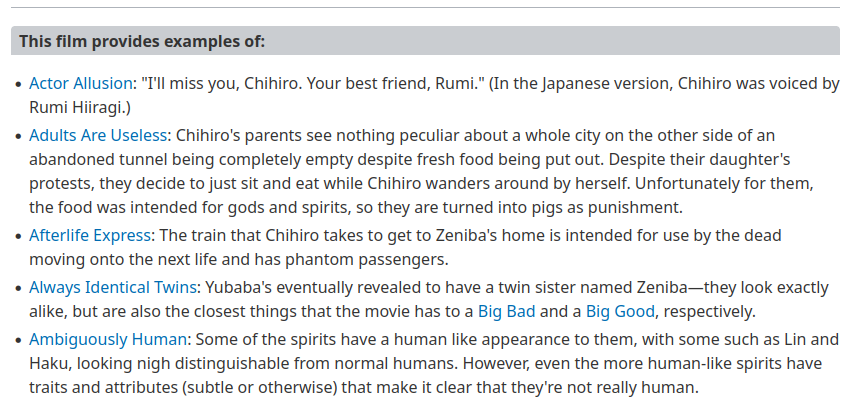
\includegraphics[width=\linewidth]{img/tropes1.png}
      \caption{Lista alfabética de \textit{tropos}.}
      \label{fig:tropelist1}
    \end{subfigure}
    \begin{subfigure}{\textwidth}
      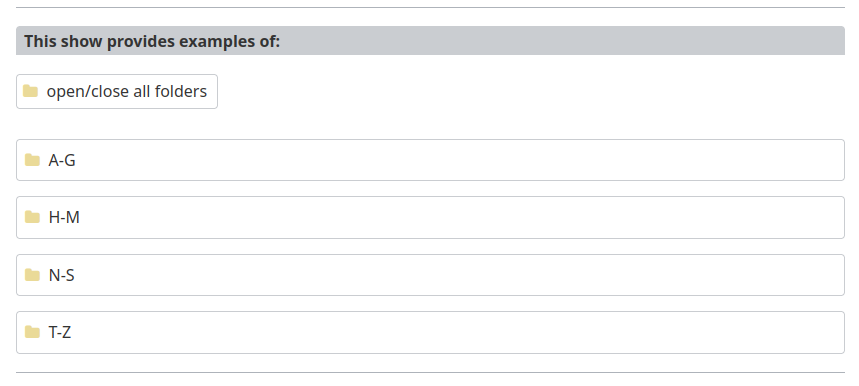
\includegraphics[width=\linewidth]{img/tropes2.png}
      \caption{\textit{Tropos} listados en carpetas.}
      \label{fig:tropelist2}
    \end{subfigure}
    \begin{subfigure}{\textwidth}%
      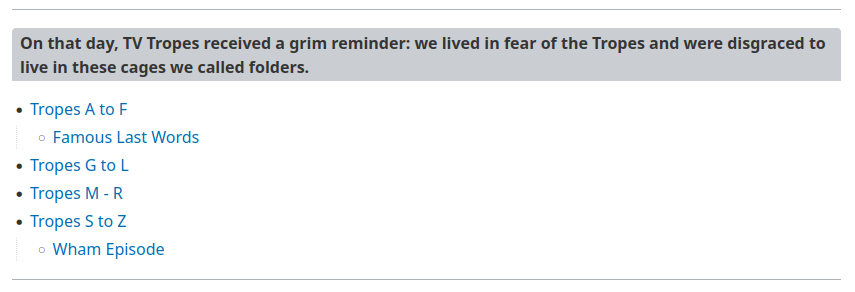
\includegraphics[width=\linewidth]{img/tropes3.png}
      \caption{\textit{Tropos} listados en sub páginas.}
      \label{fig:tropelist3}
    \end{subfigure}
    \caption{Formas más comunes de presentar los \textit{tropos}
    de una obra en TvTropes.}
    \label{fig:tropelist}
\end{figure}

En cuanto a las sub páginas dentro de una obra, estas pueden ser muchas o pocas
según la obra, ya que, también las crea la comunidad. Cualquiera de estas sub
páginas busca dar información interesante relacionada con una obra. En este
caso, están centradas en distintas temáticas o con distintos objetivos y, por
tanto, presentan información que puede ser novedosa. Existen varias muy
frecuentes, como \textit{Laconic}, que da una descripción muy breve de la obra
referenciando varios \textit{tropos} que generalmente no suelen aparecer en la
lista principal, \textit{TearJerker}, que referencia mediante \textit{tropos}
aspectos tristes de la obra, o \textit{Trivia}, que presenta curiosidades sobra
la obra y \textit{tropos} que tienen que ver con esas curiosidades. Otra de las
sub páginas más destacables es la llamada
YMMV\footnote{\url{https://tvtropes.org/pmwiki/pmwiki.php/YMMV/HomePage}}, la
cual contiene otros \textit{tropos} que no toda la comunidad identifica como
correctos o con el mismo significado y, por tanto, no corresponden en la página
principal, que lista los que no tienen diferencias de opinión. Definir todas las
sub páginas de cada obra es imposible, por lo que el \textit{scraper} debe saber
identificar la sección en la que aparecen todas estas páginas, explorarlas y
buscar enlaces de \textit{tropos}. En cualquier caso, en todas ellas la
prioridad es identificar el elemento \texttt{<div>} principal que contiene la
información de la sub página y buscar todas las etiquetas de enlace a
\textit{tropos}. Salvo \textit{Laconic}, que es un pequeño texto, el resto
suelen ser todas siempre del mismo tipo: dos secciones separadas de un pequeño
resumen de la sección (que también incluye referencias a \textit{tropos}) y
varias listas con otros ejemplos nuevos de \textit{tropos}. Esas listas están
separadas generalmente por elementos de \textit{header} que cambian según la
obra, pero donde el \textit{tropo} está incluido en el propio texto y no al
principio de él. Se pueden ignorar los \textit{headers} y simplemente buscar los
elementos de lista. Se puede ver, de forma general, un esquema de cómo son las
sub páginas de una obra en la figura \ref{fig:subpage}.

\begin{figure}[!h]
  \centering
  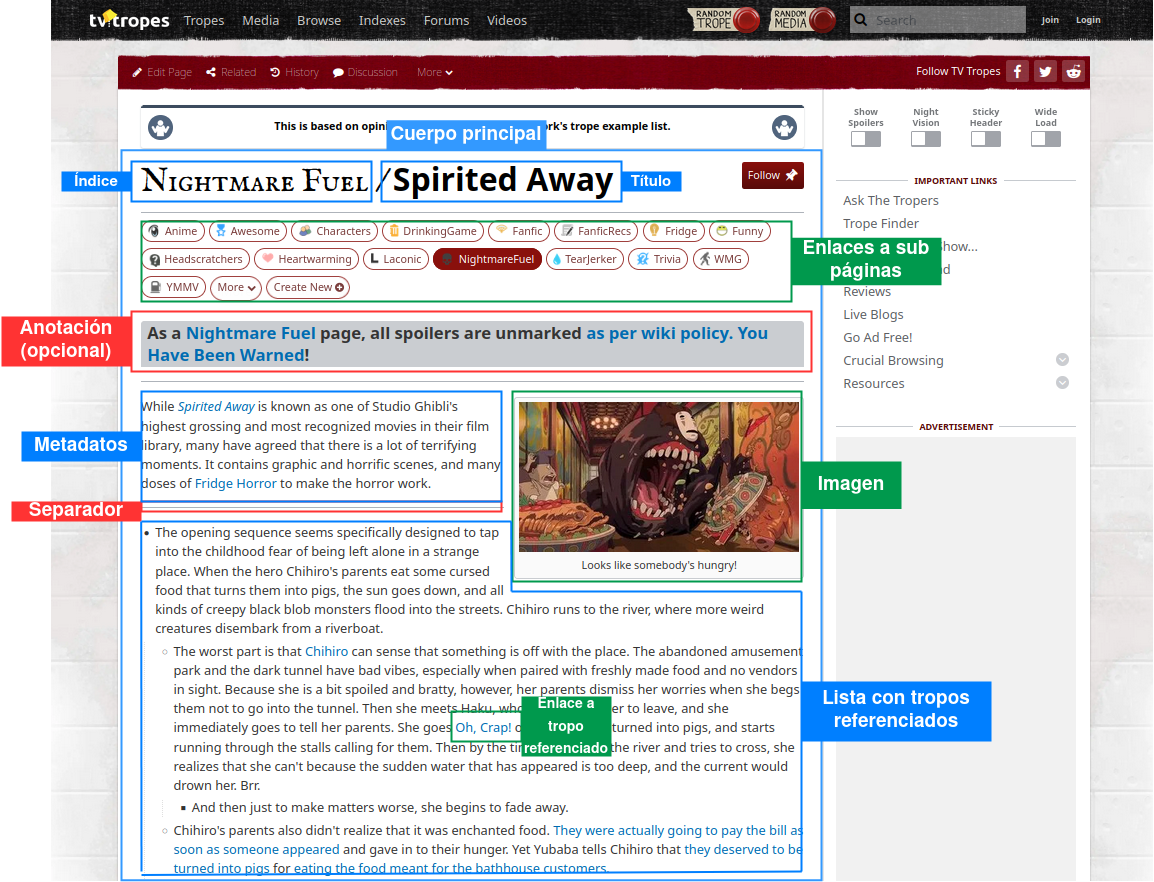
\includegraphics[width=\textwidth]{img/esquema-subpagina.png}
  \caption{Esquema de las secciones de una sub página de una obra en TvTropes.}
  \label{fig:subpage}
\end{figure}

Identificar cuándo se hace referencia a un \textit{tropo}, independientemente de
la página, es sencillo puesto que siempre son hipervínculos con la clase CSS
``\textit{twikilink}'' que, además, siguen el mismo estilo de URL que se ha
visto anteriormente. El \textit{scraper} debe buscar, siempre dentro de la misma
página de la obra, todas las secciones y sub páginas que puedan contener un
hipervínculo de tipo ``\textit{twikilink}'', extraer el nombre del
\textit{tropo} y añadirlo sin repetir.

Finalmente, se resumen los puntos principales que se deducen de este análisis de
TvTropes:
\begin{itemize}
    \item Se considera que todos los \textit{tropos} de una obra audiovisual son
    la suma de todos los que aparecen listados en la página principal, los que
    aparecen referenciados en las distintas sub páginas dentro de la propia obra
    y los que aparecen referenciados en cualquier texto, ya sea el resumen de la
    obra o la descripción de otro \textit{tropo}.
    \item Un \textit{tropo} se identifica al ser una etiqueta HTML \texttt{<a
    class=``twikilink''>}. Su URL es del tipo
    \texttt{https://tvtropes.org/pmwiki/pmwiki.php/Main/} más su nombre en
    estilo \textit{CamelCase}, sin embargo, no todas las páginas con este tipo
    de URL son necesariamente \textit{tropos}.
    \item Existen índices que contienen completamente todos los tropos y obras
    audiovisuales separadas por tipo, listados alfabéticamente y sin confusión
    de pertenecer a cualquier otra categoría. Por tanto, se sabe sin lugar a
    dudas si una página es un \textit{tropo} si está contenido en ese índice.
    \item Se respetarán los nombres que usa TvTropes para almacenar cada obra
    según su tipo de \textit{media}. Extraer dentro de la página de una obra el
    índice al que pertenece permitirá distinguir obras con mismo nombre que son
    de distinto tipo.
    \item La información a extraer en una página de una obra se encuentra
    contenida en el cuerpo principal (figura \ref{fig:tvtropes-work}), punto de
    partida del \textit{scraper}, que contiene varias etiquetas, clases e
    identificadores fácilmente identificables al ser siempre los mismos
    independientemente de la página. De la página de una obra se puede sacar, en
    orden: el índice al que pertenece, su título, un resumen con metadatos y
    \textit{tropos} referenciados, una lista principal de sus \textit{tropos} y
    sub páginas a las que habrá que acceder para identificar otros
    \textit{tropos} listados. Esta información de metadatos sirve para
    satisfacer la historia de usuario
    \href{https://github.com/jlgallego99/TropesToGo/issues/8}{[HU03]},
    eliminando la ambigüedad entre obras, y la historia
    \href{https://github.com/jlgallego99/TropesToGo/issues/9}{[HU04]} y
    \href{https://github.com/jlgallego99/TropesToGo/issues/46}{[HU07]}, para
    saber si la página ha tenido cambios y actualizar los datos.
    \item No es necesario entrar dentro de la página de un \textit{tropo} y
    explorar su código HTML, puesto que, esta solo contiene una descripción de
    este y algunos ejemplos de obras que lo contienen. No es necesario explorar
    esas obras porque ya se encontrarán desde los índices.
    \item No es necesario el uso de un motor de JavaScript en ninguna de las
    páginas, puesto que, toda la información que nos interesa está ya contenida
    en el HTML. En las páginas en las que aparecen contenidos al interaccionar
    con botones o menús desplegables, ese contenido está ya codificado en el
    HTML y el código JavaScript únicamente lo pone visible o invisible.
\end{itemize}

Todas estas características que se han analizado en las páginas de TvTropes
permitirán poder orientar una estrategia de extracción de información con el
\textit{scraper} y que este sepa identificar cuándo una página es extraíble, ya
que sabrá si la estructura de la página que está analizando se adapta a la
información que tiene codificada. Hay que tener en cuenta que todo lo analizado
en este capítulo son generalidades que comparten gran parte de las páginas de
TvTropes. Existen muchas excepciones que se irán encontrando durante el propio
proceso de desarrollo y que se estudiará en el próximo capítulo cómo proceder
con ellas.